\section{Geographical Plot: Visualizing Spatial Data}

In climate data analysis, geographical visualization plays a crucial role in understanding spatial variations across regions. Spatial data—such as district boundaries—can be combined with climate variables like temperature and precipitation to generate meaningful visual maps. These maps help reveal regional patterns that might not be obvious through tables or charts.

By visually overlaying climate information on geographic regions, researchers can detect hotspots, identify vulnerable areas, and observe spatial trends over time. Such visual tools enhance decision-making for climate adaptation strategies, regional planning, and policy development. Moreover, they improve the communication of complex climate data to stakeholders, including policymakers and the general public.

In this section, we demonstrate how to visualize spatial climate data using the \texttt{ggplot2} and \texttt{sf} packages in R. We utilize a shapefile representing the administrative boundaries of Nepal’s districts and merge it with district-level climate summaries to create intuitive thematic maps.

The shapefile provides the spatial structure (geometry) of the districts, while the associated dataset includes numerical climate values, such as average temperature and average precipitation for each district. Once merged, this combined data is plotted on a map, where color gradients represent climate intensity.

These visualizations offer a powerful way to interpret and communicate geographic patterns in climate data. They are especially useful in climate vulnerability assessment, disaster preparedness, and resource planning.

\subsection*{Shapefile Source}

The shapefile used for the geographical plots was obtained from Open Data Nepal. You can download it from the following link:

\href{https://opendatanepal.com/dataset/new-political-and-administrative-boundaries-shapefile-of-nepal}{Download shapefile of Nepal from here}

A typical shapefile set consists of multiple files including \texttt{.shp}, \texttt{.shx}, \texttt{.dbf}, \texttt{.prj}, \texttt{.cpg}, and \texttt{.qpj}.  These files work together to store not only the boundary shapes but also the related attributes and coordinate information required for accurate mapping.

In this project, the shapefile was essential for creating district-wise maps to visualize climate variables like temperature and precipitation. Before using the shapefile in R, it was loaded using spatial packages such as sf , and then joined with climate datasets based on matching district names. This allowed for layered visualizations where climate trends could be examined within their real-world geographic context


\subsection*{Required R Packages}

To run the spatial data visualizations and maps in this chapter, the following R packages must be installed and loaded:
\begin{itemize}
  \item ggmap – for base map overlays and geospatial mapping
  \item sf – for handling simple feature (spatial) data 
  \item rnaturalearth and rnaturalearthdata – for accessing natural earth map data

Use the following R commands to install and load the packages:

\end{itemize}
\begin{verbatim}
install.packages("ggmap")
install.packages("sf")
library(sf)
install.packages(c("rnaturalearth", "rnaturalearthdata"))
library(rnaturalearth)
library(rnaturalearthdata)
\end{verbatim}

\subsection*{Preparing the Shapefile for Merging}

After loading the shapefile containing Nepal’s district boundaries, the next step is to examine its structure and identify the column containing district names. This is necessary for merging the spatial data with the corresponding climate data.

\begin{verbatim}
# Load the new Nepal district shapefile
nepal_districts <- st_read("/content/shapes")

# Check column names in each dataset
colnames(nepal_districts)
\end{verbatim}

% Figure here ----------------------------
\begin{figure}[h]
\centering

\includegraphics[width=1.02\textwidth]{figures/column_names.jpg}
\caption{Column names in shapefile}
\label{fig:shapefile_columns}
\end{figure}

Upon inspecting the column names, identify the one that corresponds to district names. Here, the relevant column is \texttt{dist\_name}, which should be renamed to match the corresponding column in the climate dataset (\texttt{District}):

\begin{verbatim}
# Rename the district name column for consistency
nepal_districts <- nepal_districts %>% rename(District = dist_name)
\end{verbatim}

This ensures consistency between the spatial dataset and the climate dataset, allowing them to be merged correctly based on the \texttt{District} column.

\subsection*{Reconciling District Names between Shapefile and Climate Dataset}

Before we can merge the shapefile data with our climate dataset, we need to make sure that the names of the districts match across both sources. This is important because even small differences in spelling or naming style can cause the merge to fail or produce incorrect results.

To check for mismatches, we first view the unique district names in each dataset:

\begin{verbatim}
# View district names
unique(nepal_districts$District)
unique(df_climate$District)

\end{verbatim}


\subsection*{Merging Spatial and Climate Data}

We calculate the average temperature and precipitation for each district from the climate dataset:

\begin{verbatim}
plot_by_district <- df_climate %>%
  group_by(District) %>%
  summarise(
    avg_temp = mean(Temp_2m, na.rm = TRUE),
    avg_precip = mean(Precip, na.rm = TRUE),
    Latitude = first(Latitude),
    Longitude = first(Longitude)
  )
\end{verbatim}

These outputs show the mismatches: names from the shapefile that don’t exist in the climate data, and vice versa.

After identifying the mismatched names, we create a mapping to fix them:

\begin{verbatim}

# Verify unmatched districts
setdiff(unique(nepal_districts$District), plot_by_district$District)

setdiff(plot_by_district$District, unique(nepal_districts$District))

#Output
"Bajhang", "Bajura", "Kalikot", "Achham", "Jajarkot", "Dolakha", "Tanahu",
"Chitwan", "Ramechhap", "Kavrepalanchok", "Bhojpur", "Khotang", "Panchthar", 
"Sindhupalchok", "Rolpa", "Pyuthan", "Kapilbastu", "Parsa", "Tehrathum",
"Rautahat", "Siraha"

"Bajang", "Chitawan", "Dolkha", "Kabhre", "Panchther", "Routahat", 
"Tanahun", "Terhathum"
\end{verbatim}

After identifying the mismatched names, we create a mapping to fix them:
\begin{verbatim}
  # Create mapping for mismatched district names
district_map <- c(
  "Bajhang" = "Bajang",
  "Chitwan" = "Chitawan",
  "Dolakha" = "Dolkha",
  "Kavrepalanchok" = "Kabhre",
  "Panchthar" = "Panchther",
  "Rautahat" = "Routahat",
  "Tanahu" = "Tanahun",
  "Tehrathum" = "Terhathum"
)

# Apply the mapping to the District column
nepal_districts <- nepal_districts %>%
  mutate(District = recode(District, !!!district_map))
\end{verbatim}

This transformation ensures that the \texttt{District} column in the shapefile matches the corresponding column in the climate data, allowing for a successful merge. The use of the \texttt{!!} operator in \texttt{recode()} allows for unpacking the named vector.

Finally, we merge the cleaned shapefile data with the summarized climate data:
\begin{verbatim}
nepal_map_data <- left_join(nepal_districts, plot_by_district, 
by = "District")
\end{verbatim}

This completes the data preparation step, combining spatial and climate information for each district. Now, we can move on to visualizing the climate data on the map of Nepal.

\subsection*{Temperature Map of Nepal}

Spatial visualization of climate data enables an intuitive understanding of regional variations. A temperature map highlights how average temperatures vary across districts, helping identify hot and cold zones. Such visual tools are essential in studying local climate impacts, regional heat stress, and potential vulnerabilities in agriculture or health sectors.

The following R code loads a shapefile of Nepal’s districts, merges it with temperature data, and visualizes average temperatures using \texttt{ggplot2}:

\begin{verbatim}
ggplot(data = nepal_map_data) +
  geom_sf(aes(fill = avg_temp), color = "black") +  # Fill districts
  geom_text(data = plot_by_district, aes(x = Longitude, 
  y = Latitude, label = District),
            size = 1.5, vjust = -0.5, color = "black") +
  scale_fill_gradient(low = "yellow", high = "red") +  # Color scale
  labs(title = "Temperature Map of Nepal", fill = "Temperature") +
  theme_minimal()
\end{verbatim}

% Figure here -------------------------
\begin{figure}[h]
\centering
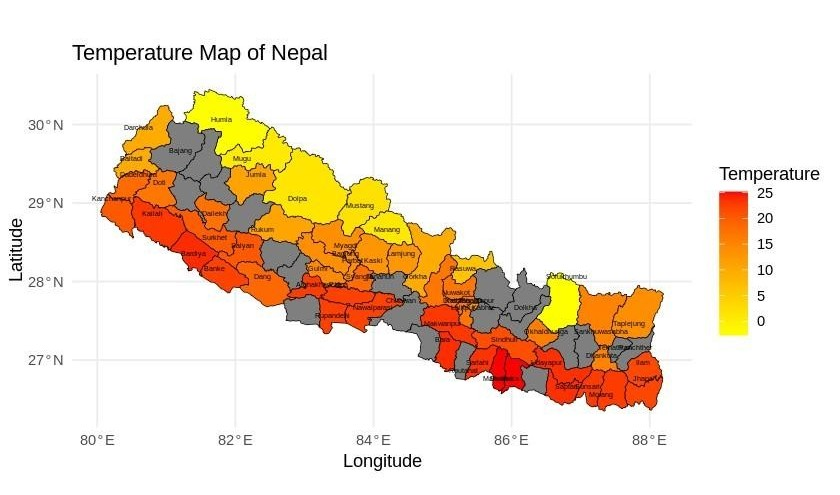
\includegraphics[width=0.6\textwidth]{figures/geo_temp.jpg}
\caption{Geoplot showing temperature distribution in Nepal}
\label{fig:temp_map_nepal}
\end{figure}

\subsection*{Precipitation Map of Nepal}

Precipitation mapping reveals the spatial distribution of rainfall, which is crucial for water resource management, agriculture, and flood risk assessment. By visualizing average precipitation at the district level, we can identify regions with excessive or insufficient rainfall, guiding decisions in irrigation planning and disaster preparedness.

\begin{verbatim}
ggplot(data = nepal_map_data) +
  geom_sf(aes(fill = avg_precip), color = "black") +  
  geom_text(data = plot_by_district, aes(x = Longitude, y = Latitude, 
  label = District),
            size = 1.5, vjust = -0.5, color = "black") +
  scale_fill_gradient(low = "skyblue", high = "blue") +  
  labs(title = "Precipitation Map of Nepal", fill = "Precipitation") +
  theme_minimal()
\end{verbatim}

% figure here ---------------------------
\begin{figure}[h]
\centering
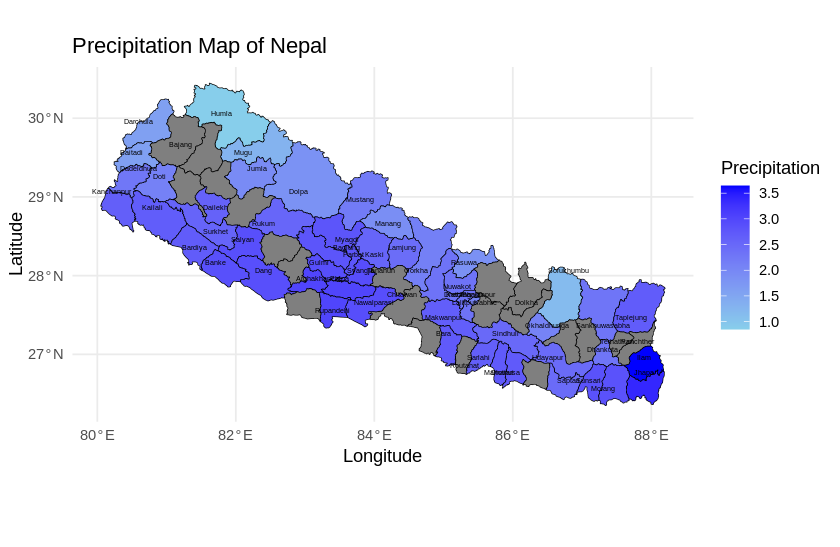
\includegraphics[width=0.6\textwidth]{figures/geo_precip.png}
\caption{Geoplot showing precipitation distribution in Nepal}
\label{fig:precip_map_nepal}
\end{figure}
